\documentclass[12pt]{article}
\usepackage{sbc/template}
\usepackage{amsmath,color,graphicx,listings,url}
\usepackage[brazil]{babel}
\usepackage[utf8]{inputenc}

\definecolor{codegreen}{rgb}{0,0.6,0}
\definecolor{codegray}{rgb}{0.5,0.5,0.5}
\definecolor{codepurple}{rgb}{0.58,0,0.82}
\definecolor{backcolour}{rgb}{0.95,0.95,0.92}

\lstdefinestyle{mystyle}{
    commentstyle=\color{codegreen},
    keywordstyle=\color{blue},
    numberstyle=\tiny\color{codegray},
    stringstyle=\color{codepurple},
    basicstyle=\footnotesize\ttfamily,
    breaklines=true,
    numbers=left,
    showstringspaces=false
}
\lstset{style=mystyle}

\sloppy

\title{RSA}

\author{Ranieri S. Althoff\inst{1}}

\address{Universidade Federal de Santa Catarina\\
Departamento de Informática e Estatística\\
Segurança em Computação}

\begin{document}

\maketitle

\section{Introdução}\label{sec:firstpage}

O RSA é um algoritmo de criptografia de chave pública, onde a chave de cifragem
é pública e diferente da chave de decifragem, que é privada. No RSA, essa
assimetria de chaves é baseada na dificuldade de fatoração do produto de dois
números primos grandes.

O nome RSA vem dos criadores Ron Rivest, Adi Shamir e Leonard Adleman e foi
publicado em 1977. Como o RSA é um algoritmo lento, ele não é frequentemente
utilizado para criptografar mensagens, em vez disso sendo usado para
criptografar chaves simétricas de outros algoritmos que são mais rápidos.

\section{Operação do RSA}

O princípio do RSA é a de que é simples encontrar três inteiros positivos $e$,
$d$ e $n$ tal que para todo $m$, $(m^{e})^{d} \equiv m \pmod{m}$ e mesmo se
sabendo $e$ e $n$ ou até mesmo $m$, é extremamente custoso encontrar $d$.

Além disso, para algumas operações é conveniente que a ordem da exponenciação
seja invertida, de forma que $(m^{d})^{e} \equiv m \pmod{m}$.

Para que Beto envie suas mensagens criptografadas, Alice transmite sua chave
pública $(n, e)$ por uma rota não necessariamente secreta e mantém sua chave
privada escondida.

\subsection{Cifragem e decifragem}

Beto transforma sua mensagem $M$ em um inteiro $m$ tal que $0 \leq m < n$ e
computa o texto cifrado $c$ usando a chave pública de Alice, correspondendo a
$c \equiv m^{e} \pmod{n}$.

Alice pode recuperar o texto claro $m$ a partir de $c$ usando sua chave privada
calculando $m \equiv c^{d} \equiv (m^{e})^{d} \pmod{n}$ o que é correto por
definição.

\subsection{Geração de chaves}

Para gerar o par de chaves RSA, utiliza-se o seguinte algoritmo:

\begin{enumerate}
    \item Escolher dois números primos distintos $p$ e $q$.
    \item Computar $n = pq$. O comprimento de $n$, expressado em bits, é o
        tamanho da chave.
    \item Computar $\phi(n) = \phi(p)\phi(q) = (p-1)(q-1) = n-(p+q-1)$.
    \item Encontrar um inteiro $e$ tal que $1 < e < \phi(n)$ e
        $gcd(e, \phi(n)) = 1$. Qualquer número primo satisfaz essa condição.
    \item Determinar $d$ como $d \equiv e^{-1} \pmod{\phi(n)}$, ou seja, $d$ é
        a inversa multiplicativa de $e$ módulo $\phi(n)$. De forma simples,
        encontrar $d$ para que $de \equiv 1 \pmod{\phi(n)}$.
\end{enumerate}

Por razões de segurança, os inteiros $p$ e $q$ devem ser aleatórios, ter
magnitude semelhante, mas diferenciar em comprimento por alguns dígitos para
dificultar a fatoração~\cite{rivest:78}. A primalidade pode ser verificada de
forma eficiente com um teste probabilístico.

É possível melhorar o desempenho utilizando um $e$ curto e com uma baixa
quantidade de bits em 1, geralmente sendo usado $e = 2^{16}+1 = 65537$. Em
geral, números na forma $2^{x}+1$ são bons candidatos. No entanto, valores
muito baixos de $e$ (por exemplo, 3) podem ser inseguros~\cite{boneh:99}.

Como os fatores comuns de $p-1$ e $q-1$ também serão fatores de $pq-1$, é
recomendado que $p-1$ e $q-1$ tenham poucos fatores comuns, de preferência
nenhum além de 2.

\subsection{Exemplo}

\begin{enumerate}
    \item Escolher dois primos distintos, por exemplo $p = 227$ e $q = 281$.
    \item Computar $n = pq$, neste exemplo $n = 227 \times 281 = 63787$. O
        comprimento em bits de $n$ é 16, neste caso.
    \item Computar $\phi(n) = \phi(p)\phi(q) = 226 \times 280 = 63280$.
    \item Encontrar $e$ relativamente primo a $\phi(n)$, como $257$.
    \item Encontrar $d$ para que $d \times 257 \equiv 1 \pmod{63280}$. O menor
        número que satisfaz essa condição é $7633$.
\end{enumerate}

A chave pública é $(n = 63787, e = 257)$ e a função de cifragem é
$c = m^{257} \pmod{63787}$. A chave privada é $(d = 7633)$ e a função de
decifragem é $m = c^{7633} \pmod{63787}$.

Se quisermos criptografar o caractere 'a', por exemplo, correspondente a $97$
em ASCII, aplicamos a função de cifragem nesse valor:

\begin{center}
    $c = 97^{257} \pmod{63787} = 10888$
\end{center}

E, para encontrar o texto original, usamos a função de decifragem no texto
cifrado:

\begin{center}
    $m = 10888^{7633} \pmod{63787} = 97$
\end{center}

\section{Código}

A classe \texttt{KeyPair} gera um par de chaves como explicado acima recebendo
como parâmetro do construtor o tamanho da chave $n$ e define $e$ como $65537$.
Depois, imprime os valores de $p$, $q$, $n$ e da chave pública e privada.

\lstinputlisting[language=Python]{rsa.py}

A saída do algoritmo usando diferentes tamanhos de chave como parâmetro pode
ser vista nas figuras anexas ao fim do documento.

\section*{Anexo - Questionário}

\begin{itemize}
    \item \textbf{O que é a função totiente de Euler?}\par
        A função totiente de Euler, ou $\phi(n)$, é uma função que conta a
        quantidade de inteiros positivos até $n$ que sejam relativamente primos
        a $n$, ou, mais formalmente, a quantidade de números inteiros $k$ no
        intervalo $1 \leq k \leq n$ onde $gcd(n, k) = 1$.
        \newline
    \item \textbf{Por que os expoentes são determinados módulo $\phi(n)$ e não
        módulo n?}\par
        O sistema RSA utiliza módulo $\phi(m)$ para determinar $e$ e $d$ com
        base na propriedade $a^{\phi(n)} \equiv 1 \pmod{n}$, o que significa
        $a^{\phi(n)+1} \equiv a \pmod{n}$ e é chamado de teorema de Euler.

        Para cifrar e decifrar usando $e$ e $d$, precisamos que
        $a^{ed} \equiv a \pmod{n}$, ou seja, precisamos que
        $ed \equiv 1 \pmod{\phi(n)}$, o que só é verdade quando ambos $e$ e $d$
        são relativamente primos a $\phi(n)$.

        Se essa relação não se manter, é impossível cifrar e decifrar um valor
        unicamente utilizando RSA, porque múltiplos valores $m$ serão cifrados
        para um mesmo valor $c$ e não é possível determinar o valor original
        na decifragem.
        \newline
    \item \textbf{O que é PKCS \#1?}
        É o primeiro padrão de uma família chamada
        \textit{Public-Key Cryptography Standards}. Esse padrão contém algumas
        definições e recomendações para a implementação do algoritmo RSA, como
        as propriedades matemáticas de chaves privadas e públicas, operações
        primitivas para cifragem e assinatura, entre outros.
        \newline
    \item \textbf{Como o RSA pode ser usado para ciframento de dados? E como
        seria usado para assinatura?}
        Para cifrar dados, é necessário usar a chave pública na mensagem em
        texto claro e enviar para o dono da chave privada. Dessa forma, apenas
        quem tem acesso a chave privada pode ler a mensagem cifrada.

        Para assinatura, o processo é inverso, onde o dono da chave privada
        cifra com a chave privada de forma que qualquer pessoa pode decifrar a
        mensagem com a chave pública e garantir que quem a cifrou foi o
        detentor da chave privada.
        \newline
    \item \textbf{Por que é importante ter bons geradores de números aleatórios
        para gerar chaves RSA?}
        O que um bom gerador de números aleatórios tem como característica é de
        gerar números aleatórios desconhecidos e aparentemente não previsíveis
        para um potencial atacante.

        Números aleatórios obtidos por um processo físico, como a leitura da
        variação da velocidade do disco, a temporização da entrada de teclas
        digitadas, etc. Uma alternativa é usar um gerador pseudo-aleatório
        alimentado por uma semente aleatória, mas um gerador desse tipo é
        necessáriamente periódico, enquanto números realmente aleatórios não
        são~\cite{rsa:09:1}.

        Um estudo conduzido em 2012~\cite{lenstra:12} utilizou chaves públicas
        disponíveis na internet e concluiu que cerca de 0.2\% de todas as
        chaves não possuem segurança por utilizarem números aleatórios de baixa
        qualidade.
        \newline
    \item \textbf{Qual seria o tamanho da chave desejável RSA nos dias atuais?}
        A escolha do tamanho de chave depende da importância do dado a ser
        cifrado. Dito isto, o maior tamanho de chave já quebrado foi de 768
        bits, portanto um tamanho de chave maior do que esse é desejável.

        Ainda assim, essa quebra levou mais de dois anos em um supercomputador
        e foi estimado em mais de 1500 anos em um computador
        comum~\cite{timmer:10}.

        A recomendação tradicional do RSA Laboratories é de se usar ao menos
        1024 bits de chave, ou usar 2048 para maior \textit{future-proofing}.
        Outra recomendação é a de Lenstra-Verheul que recomenda 952 bits no
        mínimo ou 1369 para \textit{future-proofing}~\cite{rsa:09:2}.
\end{itemize}

\bibliographystyle{sbc/sbc}
\bibliography{rsa}

\begin{figure}[ht]
    \centering
    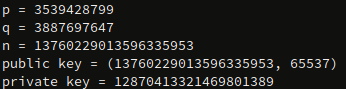
\includegraphics{rsa_64.png}
    \caption{Saída do algoritmo para 64 bits}
    \label{fig:rsa_64}
\end{figure}

\begin{figure}[ht]
    \centering
    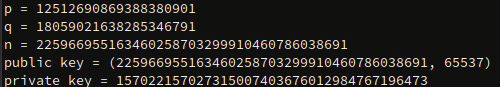
\includegraphics[width=\textwidth]{rsa_128.png}
    \caption{Saída do algoritmo para 128 bits}
    \label{fig:rsa_128}
\end{figure}

\begin{figure}[ht]
    \centering
    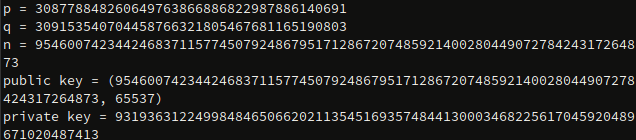
\includegraphics[width=\textwidth]{rsa_256.png}
    \caption{Saída do algoritmo para 256 bits}
    \label{fig:rsa_256}
\end{figure}

\begin{figure}[ht]
    \centering
    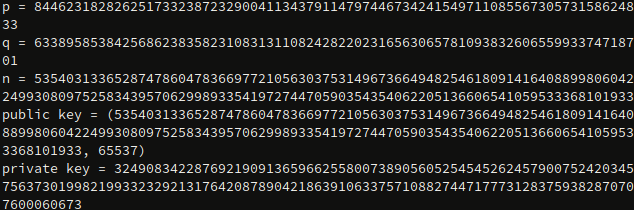
\includegraphics[width=\textwidth]{rsa_512.png}
    \caption{Saída do algoritmo para 512 bits}
    \label{fig:rsa_512}
\end{figure}

\begin{figure}[ht]
    \centering
    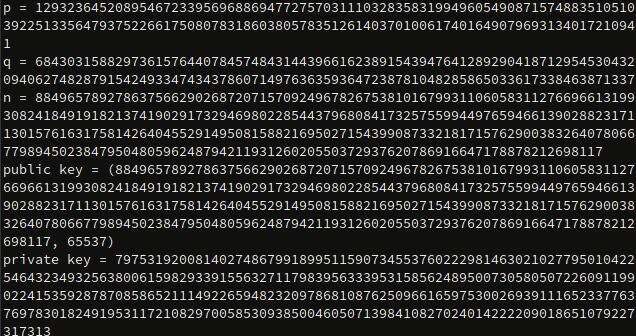
\includegraphics[width=\textwidth]{rsa_1024.png}
    \caption{Saída do algoritmo para 1024 bits}
    \label{fig:rsa_1024}
\end{figure}

\begin{figure}[ht]
    \centering
    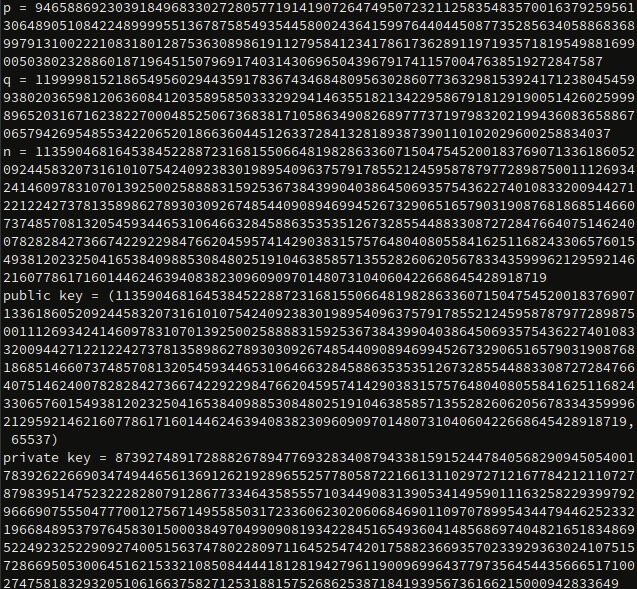
\includegraphics[width=\textwidth]{rsa_2048.png}
    \caption{Saída do algoritmo para 2048 bits}
    \label{fig:rsa_2048}
\end{figure}

\begin{figure}[ht]
    \centering
    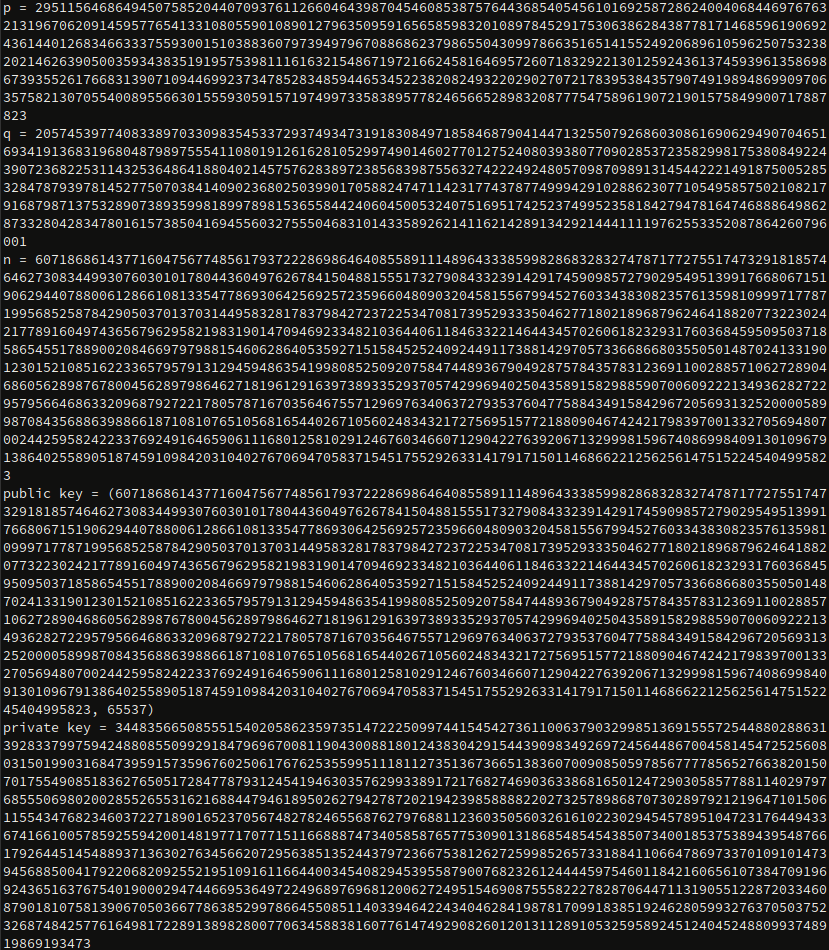
\includegraphics[width=\textwidth]{rsa_4096.png}
    \caption{Saída do algoritmo para 4096 bits}
    \label{fig:rsa_4096}
\end{figure}

\end{document}
